\documentclass[11pt]{article}
\usepackage[utf8]{inputenc}
\usepackage[T1]{fontenc}
\usepackage[spanish]{babel}
\usepackage[margin=2.5cm]{geometry}
\usepackage{amsmath,amssymb}
\usepackage{graphicx}
\usepackage{xcolor}
\usepackage{enumitem}
\usepackage{mdframed}
\usepackage{hyperref}
\hypersetup{colorlinks=true,linkcolor=blue!55!black,urlcolor=blue!55!black}

\newmdenv[
  linecolor=orange!70!black,
  backgroundcolor=orange!6,
  linewidth=0.8pt,
  roundcorner=4pt,
  skipabove=8pt,skipbelow=8pt,
  innertopmargin=6pt,innerbottommargin=6pt
]{aviso}

\title{\textbf{¿Qué buscamos con los nuevos experimentos numéricos?}\\[2pt]
\large Una explicación en palabras sencillas}
\author{Proyecto Riemann}
\date{\today}

\begin{document}
\maketitle

\noindent
Lo nuevo son, en esencia, \textbf{dos experimentos numéricos} alrededor de la
hipótesis de Riemann. Aquí explicamos \emph{la idea}, sin tecnicismos, para
entender qué se agregó y por qué.

\section*{La idea de fondo}

Hay una función objetivo, que llamamos $E$, y queremos \textbf{aproximarla}
sumando ciertas piezas $G_2, G_3, G_4, \dots$ (una por cada número entero, hasta
un tope $n$). Cada pieza va multiplicada por un peso que \emph{nosotros elegimos}
para que la aproximación quede lo mejor posible.

La pregunta clave es:
\begin{center}
\emph{¿Qué tan buena es la mejor aproximación posible con $n$ piezas?}
\end{center}
A ese ``error mínimo que queda'' lo llamamos $d_n$. Mientras más piezas usamos
(más grande $n$), mejor deberíamos aproximar, y $d_n$ debería encogerse.
\textbf{Qué tan rápido se encoge está conectado con la hipótesis de Riemann.}

\section*{Experimento 1 — Medir el error mínimo y compararlo con una constante teórica}

Lo que se agregó (\texttt{dn\_run.py}, \texttt{dn\_figure.py}, más una tabla y una
figura en el paper):

\begin{itemize}[leftmargin=*]
  \item Calculamos el error mínimo $d_n$ para muchos valores de $n$, hasta
        $n \approx 5000$ piezas.
  \item \textbf{Lo interesante:} la teoría predice que $d_n$ no baja a cero de
        cualquier forma, sino \textbf{lentamente}, siguiendo una ley concreta que
        involucra una constante famosa:
        \[
          \sum_{\rho}\frac{1}{|\rho|^2} \;=\; 2 + \gamma - \log(4\pi)\;\approx\;0.0461,
        \]
        una combinación de constantes matemáticas conocidas.
  \item \textbf{Resultado:} los números caen justo encima de esa constante,
        oscilando a su alrededor. Es decir, el cálculo \textbf{confirma la
        predicción teórica}.
  \item Como \textbf{contraste}, se probó otra receta alternativa (usar los
        coeficientes de Möbius en lugar de los pesos óptimos). Esa receta se queda
        de 5 a 15 veces peor y \textbf{no mejora} al aumentar $n$. Sirve para
        mostrar que el buen comportamiento del método óptimo \textbf{no es
        casualidad}.
\end{itemize}

\begin{aviso}
\textbf{Un detalle importante.} Al principio hubo un \emph{error sutil}
(en el prototipo \texttt{proto\_dn.py}) que hacía que el error pareciera $\sim7\%$
mejor de lo que realmente era. Se corrigió obligando a que los pesos fueran
números \emph{reales}. Por eso ahora sí coincide limpiamente con $0.0461$.
\end{aviso}

\begin{figure}[h!]
\centering
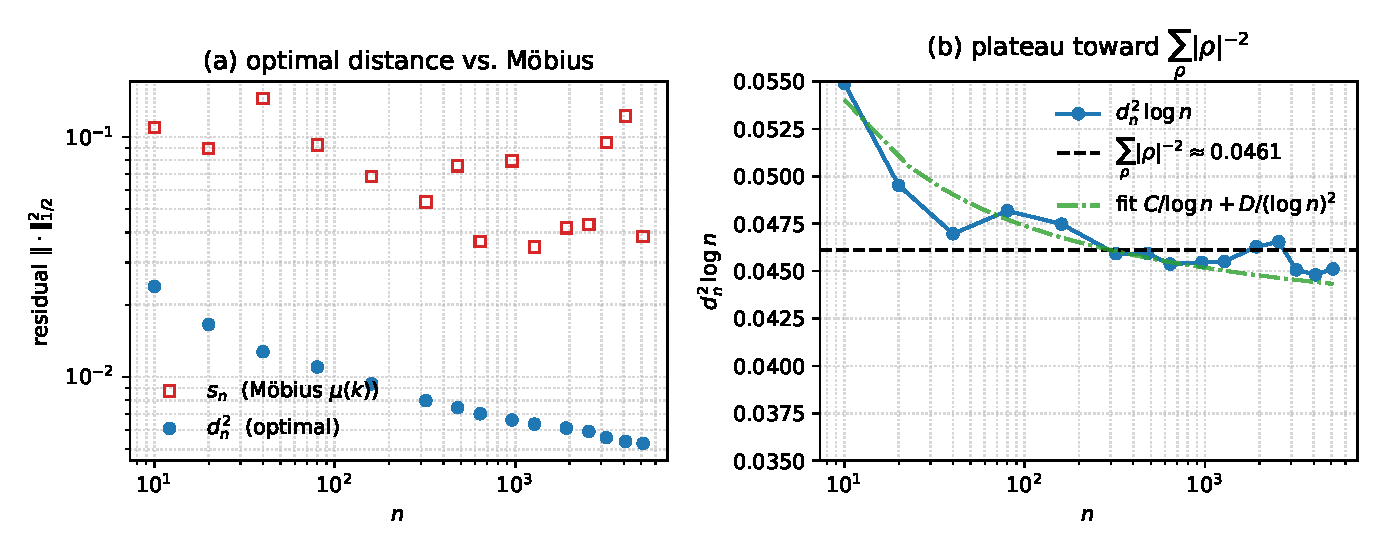
\includegraphics[width=0.85\textwidth]{fig_dn.pdf}
\caption{El error óptimo $d_n$ desciende siguiendo la ley teórica y se sienta
sobre la constante $\approx 0.0461$; la receta alternativa (Möbius) se queda muy
por encima y no mejora.}
\end{figure}

\section*{Experimento 2 — El ``barrido'' (lo más nuevo)}

Este es más ambicioso y, honestamente, \textbf{más exploratorio}
(\texttt{dn\_sweep.py}). La idea:

\begin{itemize}[leftmargin=*]
  \item Hay un parámetro $\alpha$ (piénsalo como una ``perilla''). La teoría dice
        que existe un valor crítico $\alpha_c$, y que \textbf{si ese valor crítico
        resulta ser exactamente $1/2$, entonces la hipótesis de Riemann es
        verdadera.}
  \item La expectativa era: para $\alpha < 1/2$ el error $d_n$ debería
        \textbf{estancarse} (tocar un ``piso'' y no bajar más); para
        $\alpha \ge 1/2$ debería \textbf{seguir bajando}. Ver ese cambio de
        comportamiento justo en $1/2$ sería una señal preciosa.
  \item Así que giramos la perilla $\alpha$ de $0.35$ a $0.98$ y medimos cómo se
        comporta el error en cada caso.
\end{itemize}

\paragraph{Resultado honesto.} El método \textbf{sí responde} a la perilla (a
mayor $\alpha$, el error baja más rápido, de forma suave), pero \textbf{no logra
marcar el punto crítico en $1/2$ con nitidez}. Con los $n$ que alcanzamos a
computar, una extrapolación ingenua situaría el ``quiebre'' en
$\alpha \approx 0.31$, \textbf{no} en $0.5$.

\paragraph{¿Por qué?} No porque la teoría esté mal, sino porque la convergencia es
\textbf{lentísima} (va como $1/\log n$). Con las $\sim 2500$ piezas que podemos
calcular, el error \textbf{todavía no llegó a su piso}, así que el
``estancamiento'' aún no se ve. Haría falta un $n$ fuera de nuestro alcance para
verlo bien.

\begin{aviso}
\textbf{Por eso este experimento NO entró al paper} y quedó como estudio interno.
Una lectura ingenua (``el crítico está en $0.31$'') podría malinterpretarse como
evidencia \emph{en contra} de Riemann, cuando en realidad es solo un artefacto de
usar pocas piezas.
\end{aviso}

\begin{figure}[h!]
\centering
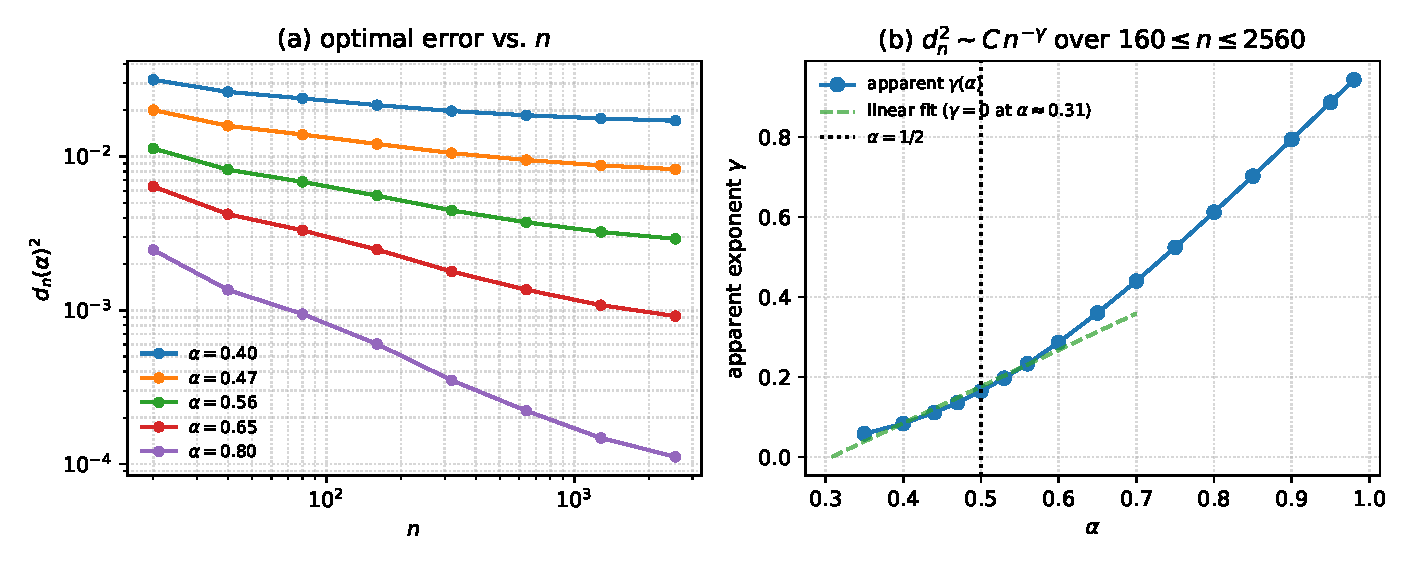
\includegraphics[width=\textwidth]{fig_sweep.pdf}
\caption{(a) La familia de curvas $d_n(\alpha)^2$: decae más rápido al crecer
$\alpha$. (b) El exponente aparente $\gamma(\alpha)$ es suave y \emph{sin quiebre}
en $\alpha=1/2$; extrapolar cruza en $\alpha\approx0.31$, un artefacto de $n$
finito.}
\end{figure}

\section*{Resumen en una frase}

\begin{itemize}[leftmargin=*]
  \item \textbf{Experimento 1:} confirma con números que el error óptimo sigue la
        ley teórica y se sienta sobre la constante $0.0461$.
        \;$\Rightarrow$\; \textbf{Entró al paper (buena evidencia).}
  \item \textbf{Experimento 2:} intentó ``ver'' el valor crítico $\alpha_c=1/2$
        girando una perilla, pero la convergencia es demasiado lenta para verlo
        con claridad. \;$\Rightarrow$\; \textbf{Quedó como nota interna honesta.}
\end{itemize}

\end{document}
